\chapter{Cookie}

Un cookie HTTP (web cookie, browser cookie) è un piccolo pezzo di dati che un server invia al browser web di un utente. Il browser può memorizzare il cookie e rinviarlo allo stesso server nelle richieste successive.\\

In genere, un cookie HTTP viene utilizzato per stabilire se due richieste provengono dallo stesso browser, ad
esempio per mantenere l'accesso di un utente. Il cookie infatti ricorda le informazioni di stato essendo che il protocollo HTTP non lo può fare poichè \textbf{stateless}.\\

I cookie vengono utilizzati principalmente per tre scopi:
\begin{itemize}
	\item \textbf{Gestione delle sessioni}: Login, carrelli della spesa, giochi o qualsiasi altra cosa il server debba ricordare.
	\item \textbf{Personalizzazione}: Preferenze dell'utente, temi e altre impostazioni.
	\item \textbf{Tracciamento}: Registrazione e analisi del comportamento degli utenti.
\end{itemize}

\section{Settare un Cookie}
I cookie vengono settati tramite gli header di risposta HTTP \textbf{Set-Cookie}. Tale header viene utilizzato per inviare un cookie dal server al browser dell'utente  in maniera tale che quest'ultimo possa inviarlo nuovamente al server nelle successive richieste all'interno dell'header HTTP \textbf{Cookie}. Se un server volesse salvare più cookie, è necessario inviare più intestazioni Set-Cookie nella stessa risposta.

Per migliorare la sicurezza del sistema (e in particolare per garantire l'invio in maniera sicura e il blocco dell'accessibilità a parti o script non previsti), i cookie mettono a disposizione una serie di attributi che vanno opportunamente settati in base allo scopo del singolo cookie:
\begin{itemize}
	\item \textbf{Expires=<date>}: È possibile specificare una data di scadenza o un periodo di tempo dopo il quale il cookie non deve essere inviato (nella realtà il cookie viene eliminato automaticamente quando scade e quindi effettivamente non lo puoi inviare perchè non esiste più). E' molto utile per i cookie di sessione in quanto, se si pensa a una banca, è bene che se l'utente non termina manualmente la sessione, i cookie devono scadere dopo qualche minuto così da non essere vulnerabili a potenziali attacchi come \textbf{CSRF}.
	\item \textbf{HttpOnly}: Impedisce a JavaScript di accedere al cookie, ad esempio tramite la proprietà \verb|Document.cookie|. Si noti che un cookie che è stato creato con HttpOnly verrà comunque inviato con richieste avviate da JavaScript, ad esempio, quando si chiama \verb|XMLHttpRequest.send()| o \verb|fetch()|. Ciò mitiga gli attacchi contro il cross-site scripting (\textbf{XSS}).
	\item \textbf{SameSite=<samesite-value>}: Controlla se un cookie viene inviato o meno con richieste cross-site, fornendo una certa protezione contro gli attacchi \textbf{CSRF} (cross-site request forgery). I possibili valori degli attributi sono:
	\begin{itemize}
		\item \textbf{Strict}: Significa che il browser invia il cookie solo per le richieste same-site, ovvero richieste provenienti dallo stesso sito che ha impostato il cookie. Se una richiesta proviene da un dominio o schema diverso (HTTP o HTTPS, anche con lo stesso dominio), non vengono inviati cookie con l'attributo ``SameSite=Strict''.
		\item \textbf{None}: significa che il browser invia il cookie sia con richieste cross-site che same-site. Anche l'attributo ``Secure'' deve essere impostato quando si imposta questo valore, in questo modo ``SameSite=None; Secure''. Se manca ``Secure'', il cookie viene rifiutato e viene registrato un errore.
		\item \textbf{Secure}: Indica che il cookie viene inviato al server solo quando viene effettuata una richiesta con lo schema https: (eccetto su localhost), e quindi è più resistente agli attacchi \textbf{MITM} (man-in-the-middle).
	\end{itemize}
\end{itemize}

\newpage

Di seguito possiamo vedere un semplicissimo esempio di come un server imposta un cookie e come questo venga rimandato dal browser al server:
\begin{figure}[ht]
	\begin{subfigure}{1\textwidth}
		\centering
		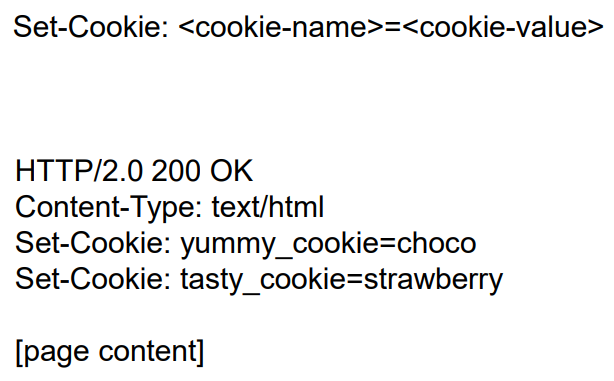
\includegraphics[width=8cm]{capitoli/web_security/imgs/set_cookie.png}  
		\caption{Set-Cookie HTTP response header.}
		\label{fig:set_cookie}
	\end{subfigure}
	
	\vspace{1.5em}
	
	\begin{subfigure}{1\textwidth}
		\centering
		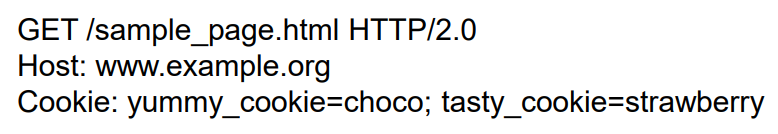
\includegraphics[width=10cm]{capitoli/web_security/imgs/send_cookie.png}  
		\caption{Cookie HTTP header.}
		\label{fig:send_cookie}
	\end{subfigure}
	\caption{Esempio ottenimento e invio di un semplice cookie.}
	\label{fig:fig}
\end{figure}